%\documentclass[11pt]{amsart}
\usepackage{geometry}                % See geometry.pdf to learn the layout options. There are lots.
\geometry{letterpaper}                   % ... or a4paper or a5paper or ... 
%\geometry{landscape}                % Activate for for rotated page geometry
%\usepackage[parfill]{parskip}    % Activate to begin paragraphs with an empty line rather than an indent
\usepackage{graphicx}
\usepackage{amssymb}
\usepackage{epstopdf}
\usepackage[noend]{algorithm2e}
\usepackage{tabularx}
\usepackage[disable]{todonotes}
%\usepackage{todonotes}
\usepackage{multirow}

\usepackage{subfig}
\usepackage{mathtools}

\DeclarePairedDelimiter\abs{\lvert}{\rvert}

%\usepackage{authblk}

%\usepackage{slashbox}
\usepackage{ amssymb }
\usepackage{tikz}
\usetikzlibrary{arrows}
\usepackage{varwidth}
\usepackage{listings}
\lstset{
  basicstyle=\ttfamily,
  mathescape
}

\newcommand\mycommfont[1]{\footnotesize\ttfamily\textcolor{gray}{#1}}
\SetCommentSty{mycommfont}


\DeclareGraphicsRule{.tif}{png}{.png}{`convert #1 `dirname #1`/`basename #1 .tif`.png}

%\newtheorem{theorem}{Theorem}
%\newtheorem{lemma}{Lemma}
%\newtheorem{proposition}{Proposition}
%\newtheorem{remark}{Remark}
\newtheorem{observation}{Observation}
%\newtheorem{definition}{Definition}

%\theoremstyle{definition}
%\newtheorem{example}{Example}

\newcommand{\targ}{\prod c^*_i}
\newcommand{\dist}{\mathcal{D}}

\newcommand{\genQ}{q}
\newcommand{\oneposQ}{\emph{1}Pos}
\newcommand{\posQ}{Pos}
\newcommand{\memQ}{\emph{Mem}}
\newcommand{\subQ}{\emph{Sub}}
\newcommand{\supQ}{\emph{Sup}}
\newcommand{\eqQ}{\emph{EQ}}
\newcommand{\pacQ}{\emph{EX}}

\newcommand{\genQi}[1]{q_{#1}}
\newcommand{\oneposQi}[1]{\emph{1}Pos_{#1}}
\newcommand{\posQi}[1]{Pos_{#1}}
\newcommand{\memQi}[1]{\emph{Mem}_{#1}}
\newcommand{\subQi}[1]{\emph{Sub}_{#1}}
\newcommand{\supQi}[1]{\emph{Sup}}
\newcommand{\eqQi}[1]{\emph{EQ}_{#1}}
\newcommand{\pacQi}[1]{\emph{EX}_{#1}}

%\newcommand{\oneposQ}{$1$-pos}
%\newcommand{\memQ}{\emph{Mem}}
%\newcommand{\subQ}{\emph{Sub}}
%\newcommand{\supQ}{\emph{Sup}}
%\newcommand{\eqQ}{\emph{EQ}}
%\newcommand{\pacQ}{\emph{PAC}}


%Complexity of Queries
\newcommand{\genC}{\#q}
\newcommand{\oneposC}{\#$1$Pos}
\newcommand{\posC}{\#Pos}
\newcommand{\memC}{\#\emph{Mem}}
\newcommand{\subC}{\#\emph{Sub}}
\newcommand{\supC}{\#\emph{Sup}}
\newcommand{\eqC}{\#\emph{EQ}}
\newcommand{\pacC}{\#\emph{EX}}

\newcommand{\genCi}[1]{\#q_{#1}}
\newcommand{\oneposCi}[1]{\#$1$Pos_{#1}}
\newcommand{\posCi}[1]{\#Pos_{#1}}
\newcommand{\memCi}[1]{\#\emph{Mem}_{#1}}
\newcommand{\subCi}[1]{\#\emph{Sub}_{#1}}
\newcommand{\supCi}[1]{\#\emph{Sup}}
\newcommand{\eqCi}[1]{\#\emph{EQ}_{#1}}
\newcommand{\pacCi}[1]{\#\emph{EX}_{#1}}



%EQ and Sub are Hard construction
\newcommand{\ntreef}{\mathfrak{c}}
\newcommand{\ntree}{\mathfrak{c}_{sub}}
\newcommand{\eqhard}{\mathfrak{C}}


\newcommand{\VC}{\mathcal{V}\mathcal{C}}



%\newcommand{\xsubQ}{\emph{XSub}}
%\newcommand{\xsupQ}{\emph{XSup}}
%\newcommand{\xeqQ}{\emph{XEQ}}
%\newcommand{\ressubQ}{\emph{resSub}}
%\newcommand{\ressupQ}{\emph{resSup}}
%\newcommand{\reseqQ}{\emph{resEQ}}




\makeatletter
\def\moverlay{\mathpalette\mov@rlay}
\def\mov@rlay#1#2{\leavevmode\vtop{%
   \baselineskip\z@skip \lineskiplimit-\maxdimen
   \ialign{\hfil$\m@th#1##$\hfil\cr#2\crcr}}}
\newcommand{\charfusion}[3][\mathord]{
    #1{\ifx#1\mathop\vphantom{#2}\fi
        \mathpalette\mov@rlay{#2\cr#3}
      }
    \ifx#1\mathop\expandafter\displaylimits\fi}
\makeatother

\newcommand{\cupdot}{\charfusion[\mathbin]{\cup}{\cdot}}
\newcommand{\bigcupdot}{\charfusion[\mathop]{\bigcup}{\cdot}}



\newcommand{\disClass}{C_{\cupdot}}


\title{Learning Cartesian-Products of Learnable Sets}
\author{}
%\date{}                                           % Activate to display a given date or no date

\begin{document}
\maketitle
%\section{}
%\subsection{}


\section{Introduction}
Traditional machine learning focuses on learning patterns from sets of (sometimes labelled) examples. 
This is useful for learning approximations of concepts. % bad sentence
However, for logical structures such as automata or propositional formulas, slight changes can result in very different behaviors. 
It is not generally possible to exactly learn these structures from just labelled examples. 

Therefore, researchers have introduced the active learning model, where the learner is allowed to make queries about the target concept to an oracle. 
Using the correct set of oracles can result in the polynomial time learnability of otherwise unlearnable sets \cite{}

Recently, exact active learning has been applied to formal synthesis, where a program is automatically generated to fit a high-level specification \cite{}. 
This has been particularly useful in Counter-Example Guided Inductive Synthesis \cite{}





\begin{figure}
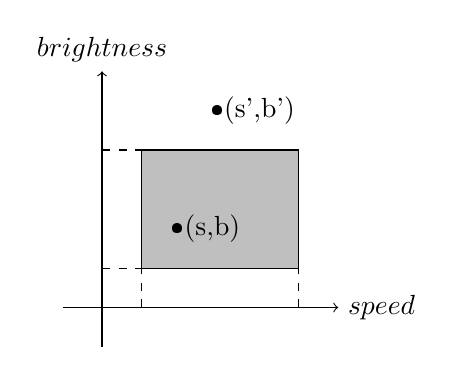
\begin{tikzpicture}
     \coordinate (BL) at (0.5,0.5);
     \coordinate (TR) at (2.5,2);
      \draw[->] (-0.5,0) -- (3,0) node[right] {$speed$};
      \draw[->] (0,-0.5) -- (0,3) node[above] {$brightness$};
      \draw [draw=black] (BL) rectangle (TR);
      \filldraw [fill=lightgray, draw=black] (BL) rectangle (TR);
      \draw[dashed] (0,0.5) -- (BL);
      \draw[dashed] (0,2) -- (0.5,2);
      \draw[dashed] (0.5,0) -- (BL);
      \draw[dashed] (2.5,0) -- (2.5,0.5);
      \draw(.75,1) node[anchor = west]{\textbullet (s,b)};
      \draw(1.25,2.5) node[anchor = west]{\textbullet (s',b')};
      %\draw (1,1) node[draw=black, anchor=south] {.};
      %\tkzDefPoint(1,1){A};
      %\tkzLabelPoint[above](A){$(1,1)$};
      
\end{tikzpicture}
\caption{The correct range of lighthouse behaviors.}
\end{figure}



\begin{table}
\begin{center}
  \begin{tabularx}{\textwidth}{| c | c | c | X | }
    \hline
    Query Name & Symbol & Complexity & Oracle Definition \\ \hline
    Single Positive Query & $\oneposQ$ & $\oneposC(c)$ & Return a fixed $x \in c^*$ \\ \hline
    Positive Query & $\posQ$ & $\posC(c)$ & Return an $x\in c^*$ that has not yet been given as a positive example (if one exists)\\ \hline
    Membership Query & $\memQ$ & $\memC(c)$ & Given string $s$, return true iff $s \in c^*$ \\ \hline
    Equivalence Query & $\eqQ$ & $\eqC$ & Given $c \in C$, return true if $c=c^*$ otherwise return $x \in (c \backslash c^*) \cup (c^* \backslash c)$\\ \hline 
    Subset Query & $\subQ$ & $\subC(c)$ & Given $c \in C$, return `true' if $c \subseteq c^*$ \mbox{  } otherwise return some $x \in c \backslash c^*$ \\ \hline
    Superset Query & $\supQ$ & $\supC(c)$ & Given $c \in C$, return `true' if $c \supseteq c^*$  otherwise return some $x \in c^* \backslash c$\\ \hline
  \end{tabularx}
\end{center}
\end{table}

\section{Important Notation}

In the following proofs, we assume we are given concept classes $C_1, C_2, \dots, C_k$ defined over sets $X_1$, $X_2$, \dots, $X_k$. 
Each $c_i$ in each $C_i$ is learnable from algorithm $A_i$ using queries to an oracle that can answer any queries in a set $Q$.  \todo{Q is almost always a singleton. Should we just call it a query instead of a set?}
For each query $q \in Q$, we say algorithm $A_i$ makes $\genC(c)$ many $q$ queries to the oracle in order to learn concept $c$, dropping the index $i$ when necessary .
We replace the term $\genC$ with a more specific term when the type of query is specified.
For example, an algorithm $A$ might make $\memC(c)$ many membership queries to learn $c$. 

Unless otherwise stated, we will assume any index $i$ or $j$ ranges over the set $\{ 1 \dots k \}$.
We write $\prod S_i$ to refer to the cartesian-product of sets $S_i$. 
Note that this is the $k$-ary cartesian product, and is not simply repeated applications of the binary cartesian product.
So for example $\prod_{i=1}^3 S_i$ equals $\{ (s_1, s_2, s_3) \mid s_1 \in S_1, s_2 \in S_2, s_3 \in S_3 \}$ and not $\{ ((s_1, s_2), s_3) \mid s_1 \in S_1, s_2 \in S_2, s_3 \in S_3 \}$
We use $S^k$ to refer to $\prod_{i=1}^k S$. 

We use vector notation $\vec{x}$ to refer to a vector of elements $(x_1,\dots, x_k)$, $\vec{x}[i]$ to refer to $x_i$, and $\vec{x}[i \leftarrow x'_i]$ to refer to $\vec{x}$ with $x'_i$ replacing value $x_i$ at position $i$. 
We define $\prod C_i := \{ \prod c_i \mid c_i \in C_i, i \in \{1,\dots,k\} \}$. 
We write $\vec{c}$ for any element of $\prod C_i $ and will often denote $\vec{c}$ by $(c_1, \dots, c_k)$ in place of $\prod c_i$. 

The results below answer the following question:
For what set of queries $Q$ does the learnability of each $C_i$ imply the learnability of $\prod C_i $ and how does the number of queries to learn $\prod C_i $ increase as a function of each $\genCi{i}(c_i)$ for each $q \in Q$?

The proofs in this paper make use of the following simple observations 
\begin{observation}
\label{subobs}
For sets $S_1, S_2, \dots, S_k$ and $T_1, T_2, \dots, T_k$, we have $\prod S_i \subseteq \prod T_i$ if and only if $S_i \subseteq T_i$ for all $i$ or $\prod S_i = \emptyset$.
\end{observation}

\begin{observation}
\label{posobs}
Fix sets $S_1, S_2, \dots, S_k$, points $x_1, x_2, \dots, x_k$ and an index $i$. 
If $x_j \in S_j$ for all $j \ne i$, then $(x_1, x_2, \dots, x_k) \in \prod S_i$ if and only if $x_i \in S_i$.
\end{observation}




\section{Negative Results}
This section introduces some fairly simple lower bounds.

We will start with a lower-bound on learnability from positive examples. 

\begin{proposition}
There exist concepts $C_1$ and $C_2$ that are each learnable from constantly many positive queries, such that $C_1 \times C_2$ is not learnable from any number of positive queries. 
\end{proposition}
\begin{proof}
Let $C_1 := \{ \{a\}, \{a,b\} \}$ and set $C_2 := \{ \mathbb{N}, \mathbb{Z} \backslash \mathbb{N} \}$. 
To learn the set in $C_1$, pose two positive queries to the oracle, and return $\{a,b\}$ if and only if both $a$ and $b$ are given as positive examples. 
To learn $C_2$, pose one positive query to the oracle and return $\mathbb{N}$ if and only if the positive example is in $\mathbb{N}$. 
An adversarial oracle for $C_1 \times C_2$ could give positive examples only in the set $\{a\} \times \mathbb{N}$. 
Each new example is technically distinct from previous examples, but there is no way to distinguish between the sets $\{a\}\times \mathbb{N}$ and $\{a,b\} \times \mathbb{N}$ from these examples. 
\end{proof}

Now we will show lower bounds on learnability from $\eqQ$, $\subQ$, and $\memQ$. 
We will see later that this lower bound is tight when learning from membership queries, but not equivalence or subset queries.


\begin{proposition}
There exists a concept $C$ that is learnable from $\genC$ many queries posed to $Q \subseteq \{ \memQ, \eqQ, \subQ \}$ such that learning $C^k$ requires $(\genC)^k$ many queries.   \todo{Should I explicitly handle infinite and finite cases separately? Should I include bigO notation on the infinite case?}
\end{proposition}
\begin{proof}
Let $C = \{ \{j\} \mid j \in \{0 \dots m\} \}$. 

We can learn $C$ in $m$ membership, subset, or equivalence queries by querying $j \in c^*$, $\{ j \} \subseteq c^*$, or $\{j\} = c^*$, respectively. 

However, a learning algorithm for $C^k$ requires more than $m^k$ queries. 
To see this, note that  $C^k$ contains all singletons in a space of size $(m+1)^k$. 

So for each subset query $\{x\} \subseteq c^*$, if $\{j\} \ne c^*$, the oracle will return $j$ as a counterexample, giving no new information.  
Likewise, for each equivalence query $\{j\} = c^*$, if $\{j\} \ne c^*$, the oracle can return $j$ as a counterexample.
Therefore, any learning algorithm must query $x \in c^*$, $\{ x \} \subseteq c^*$, or $\{x\} = c^*$ for $(m+1)^k - 1$ values of $x$
\end{proof}


\section{Positive Results}

\begin{proposition}
%Assume for each concept class $C_i$ there is a learning algorithm $A_i$ that learns each $c_i \in C_i$ in $$ superset queries (we don't assume $Q_i(c_i)$ is finite for all $c_i$). 

If $Q = \{ \supQ \}$, then there is an algorithm that learns any concept $\targ = c^*_1 \times \dots \times c^*_k  \in \prod C_i $ in $\sum \supCi{i}(c^*_i)$ queries.  
\end{proposition}
\begin{proof}
Algorithm \ref{supalg} learns $\prod C_i $ by simulating the learning of each $A_i$ on its respective class $C_i$. 
The algorithm asks each $A_i$ for superset queries $S_i$, queries the product $\prod S_i$ to the oracle, and then uses the answer to answer at least one query to some $A_i$. 
Since at least one $A_i$ receives an answer for each oracle query, at most $\sum \supCi{i}(c^*_i)$ queries must be made in total. 

 

We will now show that each oracle query results in at least one answer to an $A_i$ query (and that the answer is correct). 
The oracle first checks if the target concept is empty, if not it proceeds as normal.
At each step, the algorithm poses query $\prod S_i$ to the oracle. 
If the oracle returns 'yes' (meaning $\prod S_i \supseteq \targ$), then  $S_i \supseteq c_i^*$ for each $i$ by Observation \ref{subobs}, so the oracle answers 'yes' to each $A_i$. 
If the oracle returns 'no', it will give a counterexample $\vec{x} = (x_1,\dots,x_k) \in \targ \backslash \prod S_i$. 
There must be at least one $x_i \not\in S_i$ (otherwise, $\vec{x}$ would be in $\prod S_i$). 
So the algorithm checks $x_j \in S_j$ for all $x_j$ until an $x_i \not\in S_i$ is found. 
Since $\vec{x} \in \targ$, we know $x_i \in c_i^*$, so $x_i \in c_i^* \backslash S_i$, so the oracle can pass $x_i$ as a counterexample to $A_i$. 

Note that once $A_i$ has output a correct hypothesis $c_i$, $S_i$ will always equal $c_i$, so counterexamples must be taken from some $j \ne i$. 
\end{proof}





\begin{algorithm}[H]
\label{supalg}
\SetAlgoLined
\KwResult{Learn $\prod C_i $ from Superset Queries}
\If{$\emptyset \in C_i$ for some $i$}{
	Query $\emptyset \supseteq \targ$\;
	\If{$\emptyset \supseteq \targ$}{
		\Return{$\emptyset$}
	}
}
\For{$i = 1 \dots k$}{
	Set $S_i$ to initial subset query from $A_i$
}
 \While{Some $A_i$ has not completed}{
  Query $\prod S_i$ to oracle\;
  \eIf{$\prod S_i \supseteq c^*$ }{
   Answer $S_i \supseteq c_i^*$ to each $A_i$\;
   Update each $S_i$ to new query\;
   }{
 	Get counterexample $\vec{x} = (x_1,\dots,x_k)$
   	\For{i = 1 \dots k}{
   		\If{$x_i \not\in S_i$}{
			Pass counterexample $x_i$ to $A_i$\;
			Update $S_i$ to new query\;
			} 
  		}
 	}
	\For{i = 1 \dots k}{
		\If{$A_i$ outputs $c_i$}{
			Set $S_i := c_i$\;
		}
	}
 }
 \Return{$\prod c_i$}\;
 \caption{Algorithm for learning from Subset Queries}
\end{algorithm}






\todo{combine learning algorithm for sub, mem, and eq w/ one positive query}
\begin{proposition}
If $Q = \{\memQ\}$ and a single positive example $\vec{p} \in \targ$ is given, then $\targ$ is learnable in $k \cdot \sum \memCi{i}(c^*_i)$ membership queries. 
\end{proposition}
\begin{proof}
Algorithm \ref{linmemalg} learns by simulating each $A_i$ in sequence, moving on to $A_{i+1}$ once $A_i$ returns a hypothesis $c_i$. 
For any membership query $M_i$ made by $A_i$, $M_i \in c^*_i$ if and only if $\vec{p}[i \leftarrow M_i]\in \targ$ by Observation \ref{posobs}. 
Therefore the algorithm is successfully able to simulate the oracle for each $A_i$, yielding a correct hypothesis $c_i$. 
\end{proof}


\begin{algorithm}[H]
\label{linmemalg}
\SetAlgoLined
\KwResult{Learn $\prod C_i $ from Membership Queries and One Positive Example}
Get positive example $\vec{p}$\;
\For{$i = 1 \dots k$}{
	\While{$A_i$ has not returned a hypothesis $c_i$}{
		Get membership query $M_i$ from $A_i$\;
		Query $\vec{p}[i \leftarrow M_i]$ to oracle\;
		\eIf{Oracle returns 'yes'}{
			Pass answer $M_i \in c^*_i$ to $A_i$\;
		}{
			Pass answer $M_i \not\in c^*_i$ to $A_i$\;
		}
	}
}
\Return{$\prod c_i$} \;

 %\Return{Hi}\;%$\prod c^*_i$\;
 \caption{Algorithm for learning from Membership Queries and One Positive Example}
\end{algorithm}




%\begin{algorithm}[H]
%\label{linsubalg}
%\SetAlgoLined
%\KwResult{Learn $\prod C_i $ from Subset Queries, Membership Queries, and One Positive Example}
%\For{$i = 1 \dots k$}{
%	Set $S_i$ to initial subset query from $A_i$
%}
% \While{Some $A_i$ has not completed}{
%  Query $\prod S_i \subseteq \targ$ to oracle\;
%  \eIf{$\prod S_i \subseteq \targ$}{
%  	 Answer $S_i \subseteq c_i^*$ to each $A_i$\;
% 	 Update each $S_i$ to new query from $A_i$\;
%	}{
% 		Get counterexample $\vec{x} = (x_1,\dots,x_k)$\;
%		\For{i = 1 \dots k}{
%			Query $\vec{p}[i \leftarrow x_i] \in \targ$\;
%			\If{$\vec{p}[i \leftarrow x_i] \not\in \targ$ and $x_i \in S_i$}{
%				Pass counterexample $x_i$ to $A_i$\;
%				Update $S_i$ to new query from $A_i$\;
%			}
%		}
%	
%	}
%	\For{i = 1 \dots k}{
%		\If{$A_i$ outputs $c_i$}{
%			Set $S_i := c_i$\;
%		}
%	}
%}
%\Return{$\prod c_i$} \;
%\caption{Algorithm for learning from Subset Queries, Membership Queries, and One Positive Example}
%\end{algorithm}
%
%\begin{algorithm}[H]
%\label{lineqalg}
%\SetAlgoLined
%\KwResult{Learn $\prod C_i $ from Equivalence Queries, Membership Queries, and One Positive Example}
%\For{$i = 1 \dots k$}{
%	Set $S_i$ to initial equivalence query from $A_i$
%}
%  Query $\prod S_i = \targ?$ to oracle\;
%  \eIf{$\prod S_i = \targ$ }{
%	\Return{$\prod S_i$}	\;
%   }{
% 	Get counterexample $\vec{x} = (x_1,\dots,x_k)$\;
%	\eIf{$\vec{x} \in \targ \backslash \prod S_i$}{
%		\For{i = 1 \dots k}{
%   			\If{$x_i \not\in S_i$}{
%			Pass counterexample $x_i$ to $A_i$\;
%			Update $S_i$ to new query from $A_i$\;
%			}
%  		}
% 	}{
%		\For{i = 1 \dots k}{
%			Query $\vec{p}[i \leftarrow x_i] \in \targ$\;
%			\If{$\vec{p}[i \leftarrow x_i] \not\in \targ$ and $x_i \in S_i$}{
%				Pass counterexample $x_i$ to $A_i$\;
%				Update $S_i$ to new query from $A_i$\;
%			}
%		}
%	
%	}
%}
%\caption{Algorithm for learning from Equivalence Queries, Membership Queries, and One Positive Example}
%\end{algorithm}

\begin{proposition}
If $Q = \{\subQ\}$ and a single positive example $\vec{p} \in \targ$ is given, then $\targ$ is learnable in $\sum \subCi{i}(c^*_i)$ subset queries and $k \cdot \sum \subCi{i}(c^*_i)$ membership queries. 
\end{proposition}
\begin{proof}
The learning process is described in Algorithm \ref{linsubalg}.
For each subset query $\prod S_i \subseteq \targ$, the algorithm either returns `yes' or gives a counterexample $\vec{x} = (x_1, \dots, x_k) \in \prod S_i \backslash \targ$. 
If the algorithm returns 'yes', then by Observation \ref{subobs} $S_i \subseteq c^*_i$ for all $i$, so the algorithm can return 'yes' to each $A_i$. 
Otherwise, $\vec{x} \not\in \targ$, so there is an $i$ such that $x_i \not\in c^*_i$. 
By Observation \ref{posobs} the algorithm can query $\vec{p}[j \leftarrow x_j]$ for all $j$ until the $x_i \not\in c^*_i$ is found. 

Once the correct $c_j$ is found for any $j$, $S_j$ will equal $c_j$ for all future queries, so any counterexamples must fail on an $i \ne j$. 

Each subset query results in a correct answer being given to at least one learner $A_i$ and at most $k$ membership queries are made per subset query, yielding the desired bound on queries. 
\end{proof}

\begin{algorithm}[H]
\label{lineqalg}
\SetAlgoLined
\KwResult{Learn $\prod C_i $ from Equivalence (or Subset) Queries, Membership Queries, and One Positive Example}
\For{$i = 1 \dots k$}{
	Set $S_i$ to initial equivalence query from $A_i$
}
  Query $\prod S_i$ to oracle\;
  \eIf{$Q = \{\eqQ\}$ and $\prod S_i = \targ$ }{
	\Return{$\prod S_i$}	\;
   }{
 	Get counterexample $\vec{x} = (x_1,\dots,x_k)$\;
	\eIf{$Q = \{\eqQ\}$ and $\vec{x} \in \targ \backslash \prod S_i$}{
		\For{i = 1 \dots k}{
   			\If{$x_i \not\in S_i$}{
			Pass counterexample $x_i$ to $A_i$\;
			Update $S_i$ to new query from $A_i$\;
			}
  		}
 	}{
		\For{i = 1 \dots k}{
			Query $\vec{p}[i \leftarrow x_i] \in \targ$\;
			\If{$\vec{p}[i \leftarrow x_i] \not\in \targ$ and $x_i \in S_i$}{
				Pass counterexample $x_i$ to $A_i$\;
				Update $S_i$ to new query from $A_i$\;
			}
		}
	
	}
}
\caption{Algorithm for learning from Equivalence (or Subset)  Queries, Membership Queries, and One Positive Example}
\end{algorithm}


Finally, we study the case when $Q = \{\eqQ\}$, as described in Algorithm \ref{lineqalg}.
This algorithm works as a synthesis of the learning algorithms for Supersets and Subsets. 
When a negative example is given, the algorithm runs as in Algorithm \ref{linsubalg} for handling subset queries. 
When a positive example is given, the algorithm runs as in Algorithm \ref{supalg} for handling superset queries. 

\section{Disjoint Union}
This section discusses learning disjoint unions of concept classes. 
This is generally much easier than learning cross-products of classes, since counterexamples belong to a single dimension in the disjoint union. 
This problem uses the same notation as the cross-product case, but we denote the disjoint union of two sets as $A \cupdot B$ and the disjoint union of many sets as $\bigcupdot A_i$.  
We define the concept class of disjoint unions as $\disClass := \{ \bigcupdot c_i \mid c_i \in C_i  \}$. 

The algorithm for learning from membership queries is very easy and won't be stated here. 
Algorithm \ref{disjalg} shows the learning procedure for when $Q \in \{ \{\subQ\}, \{\supQ\}, \{\eqQ\}\}$.
The correctness of this algorithm follows from the following simple facts.
Assume we have sets $S_1,\dots,S_k$ and $T_1,\dots,T_k$.
Then $\bigcupdot S_i \subseteq \bigcupdot T_i$ if and only $S_i \subseteq T_i$ for all $i$.
Likewise $\bigcupdot S_i = \bigcupdot T_i$ if and only if $S_i = T_i$ for all $i$.



\begin{algorithm}[H]
\label{disjalg}
\SetAlgoLined
\KwResult{Learning Disjoint Unions}
\For{$i = 1 \dots k$}{
	Set $S_i$ to initial query from $A_i$
}
\While{Some $A_i$ has not terminated}{
  Query $\bigcupdot S_i$ to oracle\;
  \eIf{Oracle returns `yes' }{
	Pass 'yes' to each $A_i$\;
   	Get updated $S_i$ from each $A_i$\; 
   }{
 	Get counterexample $x_i \in X_i$ for some $i$\;
	Pass $x_i$ as counterexample to $A_i$\;
	Get updated $S_i$ from each $A_i$\; 
	}
}
\Return{$\bigcupdot S_i$}\;
\caption{Learning Disjoint Unions}
\end{algorithm}





\section{Learning with Only Membership Queries}

We have seen that learning with membership queries can be made significantly easier if a single positive example is given. 
In this section we describe a learning algorithm using membership queries when no positive example is given. 
This algorithm makes $O(max_i \{ \memCi{i}(c_i) \}^k)$ queries, matching the lower bound given in a previous section. 

For this algorithm to work, we need to assume that $\emptyset \not\in C_i$ for all $i$.
If not, there is no way to distinguish between an empty and non-empty concept. 
For example consider the classes $C_1 = \{ \{1\}, \emptyset \}$ and $C_2 = \{ \{j \} \mid j \in \mathbb{N} \}$. 
It is easy to know when we have learned the correct class in $C_1$ or in $C_2$ using membership queries. 
However, for any finite number of membership queries, there is no way to distinguish between the sets $\emptyset$ and $\{(1,j)\}$ for some $j$ that has yet to be queried.


The main idea behind this algorithm is that learning from membership queries is easy once a single positive example is found. 
So the algorithm runs until a positive example is found from each concept or until all concepts are learned. 
If a positive example is found, the learner can then run Algorithm \ref{lineqalg} for learning from membership queries and a single positive example. 


\begin{proposition}
Algorithm \ref{memonlyalg} will terminate after making $O(max_i \{ \memCi{i}(c_i) \}^k)$ queries.
\end{proposition}
\begin{proof}
The algorithm works by constructing sets $S_i$ of elements and querying all possible elements of $\prod S_i$. 
We will get our bound of $O(max_i \{ \memCi{i}(c_i) \}^k)$ by showing the algorithm will find a positive example once $| S_i | > max_i \{ \memCi{i}(c_i) \}$ for all $i$. 
Since the algorithm queries all possible elements of $\prod S_i$, it is sufficient to prove that $S_i$ will contain an element of $c_i$ once $|S_i| > \memCi{i}(c_i)$. 

Assume that each learner eventually terminates. 
%This means that for any $c_i$ in any $C_i$, either $A_i$ eventually queries a point $x \in c_i$ or the learner outputs $c_i$ after finitely many negative membership queries. 
Let $\vec{q}^i = q_1^i, q_2^i, \dots$ be the membership queries $A_i$ makes assuming it only receives negative answers from an oracle. 
If $\vec{q}^i$ is finite, then there is some set $N_i \in C_i$ that $A_i$ outputs after querying all points in $\vec{q}^i$ (and receiving negative answers). 
If $N_i$ is non-empty let $n_i$ be some element in $N_i$. 
Note that although sampling elements from a set might be expensive in general, this is only done for $N_i$ and can therefore be hard-coded into the learning algorithm. 
If $c_i = N_i$, then by our assumption that $\targ \ne \emptyset$, $N_i$ contains some $n_i$. 
So $S_i$ contains an element of $c_i$ at the start of the algorithm. 
If $c_i \ne N_i$, by our assumption that $A_i$ eventually terminates, $A_i$ must eventually query some $q_j^i \in c_i$. 
So after $j$ steps, $S_i$ contains some element of $c_i$.
Since $j < \memCi{i}(c_i)$, we have that $S_i$ contains a positive example once $| S_i | > \memCi{i}(c_i)$, completing the proof.  
\end{proof}






\begin{algorithm}[H]
\label{memonlyalg}
\SetAlgoLined
\KwResult{Learning with Membership Queries Only}
\For{$i = 1 \dots k$}{
	\eIf{$N_i$ and $n_i$ exist}{
		Set $S_i := \{n_i\}$\;
	}{
		Set $S_i := \{ \}$\; 
	}
}
Set $j = 0$\;
\While{True}{
	\For{i = \{1, \dots, k\}}{
		\If{ $|\vec{q}^i| \ge j$ }{
			$S_i := S_i \cup \{q_j^i\}$\;
		}
	}
  \For{$\vec{x} \in \prod S_i$}{
  	Query $\vec{x} \in \targ$\;
	\If{$\vec{x} \in \targ$}{
		Run Algorithm \ref{linmemalg} using $\vec{x}$ as a positive example\;	
	}
  }
  $j := j+1$\;
}
\caption{Algorithm for Learning from Membership Queries Only}
\end{algorithm}



\section{Learning Cartesian Products with Equivalence or Subset Queries is Hard}


The previous section showed that learning cross products of membership queries requires at most $O(max_i \{ \memCi{i}(c_i) \}^k)$ membership queries. 
A natural next question is whether this can be done for equivalence and subset queries. 
In this section, we answer that question in the negative. 
We will construct a class $\eqhard$ that can be learned from $n$ equivalence or membership queries but which requires at least $k^n$ queries to learn $\eqhard^k$.  

We define $\eqhard$ to be the set $\{ \ntreef(s) \mid s \in \mathbb{N}^* \}$, where $\ntreef(s)$ is defined as follows:

\[\ntreef(\lambda) = \{\lambda\} \times \mathbb{N}\]
\[\ntreef(s) = (\{s\} \times \mathbb{N}) \cup \ntree(s)\]
\[\ntree(sa) = (\{s\} \times (\mathbb{N} \backslash \{a\})) \cup \ntree(s)\]\\

For example, $\ntreef(12) = (\{12\} \times \mathbb{N}) \cup (\{1\}\times(\mathbb{N} \backslash \{2\}))\cup(\{\lambda\} \times (\mathbb{N} \backslash \{1\}))$.


An important part of this construction is that for any two strings $s,s' \in \mathbb{N}$, we have that $\ntreef(s) \subseteq \ntreef(s')$ if and only if $s = s'$. 
This implies that a subset query will return true if and only if the true concept has been found. 
Moreover, an adversarial oracle can always give a negative example for an equivalence query, meaning that oracle can give the same counterexample if a subset query were posed. 
So we will show that $\eqhard$ is learnable from equivalence queries, implying that it is learnable from subset queries. 

We we prove a lower-bound on learning $\eqhard^k$ from subset queries from an adversarial oracle. 
An adversarial equivalence query oracle can give the exact same answers and counterexamples, implying that  $\eqhard^k$ is hard to learn from equivalence queries. 

\begin{proposition}
There exist algorithms for learning from equivalence queries or subset queries such that any concept $\ntreef(s) \in \eqhard$ can be learned from $|s|$ queries. 
\end{proposition}
\begin{proof}
(proof sketch) Algorithm \ref{ntree} shows the learning algorithm for equivalence queries. 
As mentioned above, this algorithm is essentially the same for learning from subset queries. 
When learning $\ntreef(s)$ for any $s \in \mathbb{N}^*$, the algorithm will construct $s$ by learning at least one new element of $s$ per query. 
Each new query to the oracle is constructed from a string that is a substring of $s$
If a positive counterexample is given, this can only yield a longer substring of $s$.
\end{proof}


\begin{algorithm}[H]
\label{ntree}
\SetAlgoLined
\KwResult{}
Set $s = \lambda$\;
\While{True}{
	Query $\ntreef(s)$ to Oracle
	\If{Oracle returns `yes'}{
		\Return $\ntreef(s)$
	}
	\If{Oracle returns $(s',m) \in c^* \backslash \ntreef(s)$ }
	{
		Set $s = s'$\;
	}
	\If{Oracle returns $(s,m) \in \ntreef(s) \backslash c^*$}{
		Set $s = sm$\;
	}
} 
\caption{Learning $\eqhard$ from equivalence queries.}
\end{algorithm}


\subsection{Showing $\eqhard^k$ is Hard to Learn}

It is easy to learn $\eqhard$, since each new counterexample gives one more element in the target string $s$. 
When learning a concept, $\prod \ntreef(s_i)$, it is not clear which dimension a given counterexample applies to. 
Specifically A given counterexample $\vec{x}$ could have the property that $\vec{x}[i] \in \ntreef(s_i)$ for all $i \ne j$, but the learner cannot infer the value of this $j$. 
It will then proceed considering all possible values of $j$, requiring exponentially more queries for longer $s_i$. \todo{is this clear?} 
This subsection will formalize this notion to prove an exponential lower bound on learning $\eqhard^k$. 
First, we need a couple definitions. 


A concept $\prod \ntreef(s_i)$ is \emph{justifiable} if one of the following holds:
\begin{itemize}
\item For all $i$, $s_i = \lambda$
\item There is an $i$ and an $a \in \mathbb{N}$ and $w \in \mathbb{N}^*$ such that $s_i = wa$, and $\ntreef(s_1) \times \dots \times \ntreef(w) \times \dots \times \ntreef(s_k)$ \todo{need flat cross product} was justifiably queried to the oracle and received a counterexample $\vec{x}$ such that $\vec{x}[i] = (w, a)$. 
\end{itemize}

A concept is \emph{justifiably queried} if it was queried to the oracle when it was justifiable. 
\newline


The adversarial oracle works as follows:
\begin{itemize}
\item It will always answer the same query with the same counterexample.  
\item Given any query $\prod \ntreef(s_i) \subseteq c^*$, the oracle will return a counterexample $\vec{x}$ such that for all $i$, $\vec{x}[i] = (s_i, a_i)$, and $a_i$ has not been in any query or counterexample yet seen.
\end{itemize}

Consider the following example when $k = 2$. 
First, the learner queries $(\ntreef(\lambda), \ntreef(\lambda))$ to the oracle and receives a counter-example $((\lambda, 1), (\lambda, 2))$. 
The justifiable concepts are now $(\ntreef(1), \ntreef(\lambda))$ and $(\ntreef(\lambda), \ntreef(2))$. 
The learner queries $(\ntreef(1), \ntreef(\lambda))$ and receives counterexample  $((1, 3), (\lambda, 4))$. 
 The learner queries $(\ntreef(\lambda), \ntreef(2))$ and receives counterexample $((\lambda, 5), (2, 6))$.
The justifiable concepts are now  $(\ntreef(1), \ntreef(4))$, $(\ntreef(1 \cdot 3), \ntreef(\lambda))$, $(\ntreef(5), \ntreef(2))$ and $(\ntreef(\lambda), \ntreef(2 \cdot 6))$.  
At this point, the only possible solutions constructible from strings of length $1$ are $(\ntreef(1), \ntreef(4))$ and $(\ntreef(5), \ntreef(2))$. 





For any strings $s,s' \in \mathbb{N}^*$, we write $s \le s'$ if $s$ is a substring of $s'$, and we write $s < s'$ if $s \le s'$ and $s \ne s'$.
We say that the \emph{sum of string lengths} of a concept $\prod \ntreef(s_i)$ is of size $r$ if $\sum |s_i| = r$

The following simple proposition can be proven by induction on sum of string lengths.

\begin{proposition}
\label{subjust}
Let $\prod \ntreef(s_i)$ be a justifiable concept. 
Then for all $w_i \le s_i$, $\prod \ntreef(w_i)$ has been queried to the oracle.
\end{proposition}

\begin{proposition}
\label{numjustconc}
If all justified concepts $\prod \ntreef(s_i)$ with sum of string lengths equal to $r$ have been queried, then there are $k^{r+1}$ justified queries whose sum of string lengths equals $r+1$
\end{proposition}
\begin{proof}
This proof follows by induction on $r$. 
When $r=0$, the concept $\prod \ntreef(\lambda)$ is justifiable.%has been queried and a counterexample $\vec{x}$ has been given.
%Then for all $i$, the concept which is $\ntreef(\lambda)$ at all $j \ne i$ and $\ntreef(\vec{x}[i])$ is justifiable (there are $k$ such $i$.
For induction, assume that there are $k^r$ justifiable queries with sum of string lengths equal to $r$. 
By construction, the oracle will always chose counterexamples with as-yet unseen values in $\mathbb{N}$. 
So querying each concept $\prod \ntreef(s_i)$ will yield a counterexample $\vec{x}$ where for all $i$, $\vec{x}[i] = (s_i, a_i)$ for new $a_i$.
Then for all $i$, this query creates the justifiable concept $\prod \ntreef(s'_i)$, where $s'_j = s_j$ for all $j \ne i$ and $s'_i = \ntreef(s_i \cdot a_i)$.
Thus there are $k^{r+1}$ justifiable concepts with sum of string lengths equal to $r+1$.
\end{proof}

\begin{theorem}
Any algorithm learning $\eqhard^k$ from subset (or equivalence) queries requires at least $k^r$ queries to learn a concept $\prod \ntreef(s_i)$, whose sum of string lengths is $r$.
Equivalently, the algorithm takes $k^{\sum \genCi{i}}$ subset (or equivalence) queries.
\end{theorem}
\begin{proof}
Assume for contradiction that an algorithm can learn with less than $k^r$ queries and let this algorithm converge on some concept $c = \prod \ntreef(s_i)$ after less than $k^r$ queries. \todo{explain how to assume the oracle will never return "true" on a query.}
%We will construct another concept $c' = \prod \ntreef(s'_i)$ that is consistent with all given oracle answers, but whose sum of string lengths is less than $r$.
Since less than $k^r$ queries were made to learn $c$, by Proposition \ref{numjustconc}, there must be some justifiable concept $c' = \prod \ntreef(s'_i)$ with sum of string lengths less than or equal to $r$ that has not yet been queried.
By proposition \ref{subjust} we can assume without loss of generality that for all $w_i \le s_i'$, $\prod \ntreef(w_i)$ has been queried to the oracle.
We will show that $c'$ is consistent with all given oracle answers, contradicting the claim that $c$ is the correct concept. 
Let $c_v = \prod \ntreef{v_i}$ be any concept queried to the oracle, and let $\vec{x}$ be the given counterexample.
If for all $i$, $v_i \le s'_i$, then by construction, there is an $i$ with $\vec{x}[i] = (v_i, a_i)$ such that $v_i \cdot a_i \le s'_i$, so $\vec{x}$ is a valid counterexample.
Otherwise, there is an $i$ such that $v_i \not\le s'_i$. 
So $\{v_i\} \times \mathbb{N}  \cap \ntreef(s'_i) = \emptyset$, so $\vec{x}$ is a valid counterexample. 
Therefore, all counterexamples are consistent with $c'$ being correct concept, contradicting the claim that the learner has learned $c$. 
\end{proof}






\tikzset{
  treenode/.style = {align=center, inner sep=0pt, text centered,
    font=\sffamily},
    cnode/.style = {treenode, circle, black, font=\sffamily\bfseries, draw=black, text width=2.2em},
    elip/.style = {treenode,  draw=none, black, font=\sffamily\bfseries,  text width=2em},
    edge_style/.style={draw=black}
%  arn_n/.style = {treenode, circle, white, font=\sffamily\bfseries, draw=black,
%    fill=black, text width=1.5em},% arbre rouge noir, noeud noir
%  arn_r/.style = {treenode, circle, red, draw=red, 
%    text width=1.5em, very thick},% arbre rouge noir, noeud rouge
%  arn_x/.style = {treenode, rectangle, draw=black,
%    minimum width=0.5em, minimum height=0.5em}% arbre rouge noir, nil
}

\begin{tikzpicture}[->,>=stealth',level/.style={sibling distance = 5cm/#1,
  level distance = 1.5cm}] 
\node[cnode] at (0, 0)   (lam) {$\ntreef(\lambda)$};
\node[cnode] at (-2, -2)   (1) {$\ntreef(1)$};
\node[cnode] at (0, -2)   (2) {$\ntreef(2)$};
\node[elip] at (3, -2)   (elp1) {$...$};
\node[cnode] at (-3.5, -4)   (11) {$\ntreef(11)$};
\node[cnode] at (-2, -4)   (12) {$\ntreef(12)$};
\node[elip] at (1, -4)   (elp2) {$...$};

 \draw[edge_style]  (lam) edge node[above left]{$(\lambda,1)$} (1);
 \draw[edge_style]  (lam) edge node[right]{$(\lambda,2)$} (2);
 \draw[edge_style]  (lam) edge (elp1);
 \draw[edge_style]  (1) edge node[above left]{$(1,1)$} (11);
 \draw[edge_style]  (1) edge node[right]{$(1,2)$} (12);
 \draw[edge_style]  (1) edge (elp2);

%\node [cnode] {}
%    child{ node [cnode] {$\ntreef(1)$}
%            child{ node [cnode] {$\ntreef(11)$} edge from parent node[above left] {$(1, 1)$}}
%            child{ node [cnode] {$\ntreef(12)$} edge from parent node[above right] {$(1, 2)$}}
%              edge from parent node[above left] {$(\lambda, 1)$}                             
%    }
%    child { node [cnode] {$\ntreef(2)$} edge from parent node[above left] {$(\lambda, 2)$}}
%    child { node [cnode] {$\ntreef(2)$} }
%; 
\end{tikzpicture}



%\begin{center}
%\begin{tabular}{ |c|c|c|c|c|c|c|c| } 
%Queries allowed & Complexity\\ Measured & \posQ & \supQ & \memQ & \subQ & \eqQ \\
%\hline
%Q & \genC & Not Possible & $\sum \supCi{i}$ & $(max_i\{\memCi{i}\})^k$ & $k^{\sum \subCi{i}}$ & $k^{\sum \eqCi{i}}$\\
%\multirow{2}{4em}{$Q \cup \{\memQ, \oneposQ\}$} & \memC & Not Possible & $0$ & same as below& $k \sum \subCi{i}$ & $k \sum \eqCi{i}$\\
%\genC & Not Possible & $\sum \supCi{i}$ & $\sum \memCi{i}$ & $\sum \subCi{i}$ & $\sum \eqCi{i}$\\
%\hline
%\end{tabular}
%\end{center}

\begin{figure}
\begin{center}
\renewcommand{\arraystretch}{1.5}
\begin{tabular}{ |c|c|c|c| } 
\cline{2-4}
\multicolumn{1}{c|}{} & Only $Q$ & \multicolumn{2}{c|}{$Q$ with $\memQ$ and $\oneposQ$} \\
\multicolumn{1}{c|}{} & \genC & \memC & \genC \\
\hline
\posQ & Not Possible  & Not Possible & Not Possible \\
\hline
\supQ & $\sum \supCi{i}$ & $0$ & $\sum \supCi{i}$\\
\hline
\memQ & $(max_i\{\memCi{i}\})^k$ & $\sum \memCi{i}$ & $\sum \memCi{i}$ \\
\hline
\subQ & $k^{\sum \subCi{i}}$ & $k \sum \subCi{i}$  & $\sum \subCi{i}$ \\
\hline
\eqQ  &$k^{\sum \eqCi{i}}$ &  $k \sum \eqCi{i}$ &  $\sum \eqCi{i}$\\
\hline
\end{tabular}
\renewcommand{\arraystretch}{1}
\end{center}
\caption{
Final collection of runtimes. 
The rows represents the set $Q$ of queries needed to learn each $C_i$.  
The columns determine whether the cross product is learned from queries in just $Q$ or $Q \cup \{\memQ, \oneposQ\}$. 
In the latter case, the column is separated to track the number of membership queries and queries in $Q$ that are needed.
}
\end{figure}

%\begin{center}
%\begin{tabular}{ |c|c|c|c| } 
%\hline
%col1 & col2 & col3 \\
%\hline
%\multirow{3}{4em}{Multiple row} & cell2 & cell3 \\ 
%& cell5 & cell6 \\ 
%\cline{2-3} & cell8 & cell9 \\ 
%\hline
%\end{tabular}
%\end{center}



\end{document}  